\markboth{State of the art}{State of the art}
\chapter{State of the art (hyphenation \mbox{in the table of contents} is deactivated)}
\label{cha:State of the art}

%%%%%%%%%%%%%%%%%%%%%%%%%%%%%%%%%%%%%%%%%%%%%%%%%%

\section{Literature and research}
\label{sec:Literature and research}
Lorem ipsum \citet{Book2021} dolor sit amet, consetetur sadipscing elitr, sed diam nonumy eirmod tempor invidunt ut labore et dolore magna aliquyam erat, sed diam voluptua. At vero eos et accusam et justo duo dolores et ea rebum. Stet clita kasd gubergren, no sea takimata sanctus est Lorem ipsum dolor sit amet. Lorem ipsum dolor sit amet, consetetur sadipscing elitr, sed diam nonumy eirmod tempor invidunt ut labore et dolore magna aliquyam erat, sed diam voluptua. At vero eos et accusam et justo duo dolores et ea rebum. ``Stet clita kasd gubergren, no sea takimata sanctus est Lorem ipsum dolor sit amet.''~\citep[p. 30]{Book2021}

\subsection{Disciplinary development}
\label{ssec:Disciplinary development}
%Lorem ipsum dolor sit amet, consetetur sadipscing elitr, sed diam nonumy eirmod tempor invidunt ut labore et dolore magna aliquyam erat, sed diam voluptua. At vero eos et accusam et justo duo dolores et ea rebum. Stet clita kasd gubergren, no sea takimata sanctus est Lorem ipsum dolor sit amet. Lorem ipsum dolor sit amet, consetetur sadipscing elitr, sed diam nonumy eirmod tempor invidunt ut labore et dolore magna aliquyam erat, sed diam voluptua. At vero eos et accusam et justo duo dolores et ea rebum. Stet clita kasd gubergren, no sea takimata sanctus est Lorem ipsum dolor sit amet.

\vspace{3mm}

\subsubsection{Genesis of scientific concepts}
\label{sssec:Genesis of scientific concepts}
Lorem ipsum dolor sit amet, consetetur sadipscing elitr, sed diam nonumy eirmod tempor invidunt ut labore et dolore magna aliquyam erat, sed diam voluptua. At vero eos et accusam et justo duo dolores et ea rebum. Stet clita kasd gubergren, no sea takimata sanctus est Lorem ipsum dolor sit amet. Lorem ipsum dolor sit amet, consetetur sadipscing elitr, sed diam nonumy eirmod tempor invidunt ut labore et dolore magna aliquyam erat, sed diam voluptua. At vero eos et accusam et justo duo dolores et ea rebum. Stet clita kasd gubergren, no sea takimata sanctus est Lorem ipsum dolor sit amet.

Lorem ipsum dolor sit amet, consetetur sadipscing elitr, sed diam nonumy eirmod tempor invidunt ut labore et dolore magna aliquyam erat, sed diam voluptua. At vero eos et accusam et justo duo dolores et ea rebum. Stet clita kasd gubergren, no sea takimata sanctus est Lorem ipsum dolor sit amet. Lorem ipsum dolor sit amet, consetetur sadipscing elitr, sed diam nonumy eirmod tempor invidunt ut labore et dolore magna aliquyam erat, sed diam voluptua. At vero eos et accusam et justo duo dolores et ea rebum. Stet clita kasd gubergren, no sea takimata sanctus est Lorem ipsum dolor sit amet.\footnote{
	First paragraph: This footnote has a one-digit footnote number with a fixed distance between the footnote number and the footnote text. This footnote spans two lines.

	Second paragraph: The indentation depth of the second paragraph is identical to the indentation depth of the first paragraph.
} % End of footnote

\subsubsection*{Subheading}
\label{sssec:Subheading}
Lorem ipsum dolor sit amet, consetetur sadipscing elitr, sed diam nonumy eirmod tempor invidunt ut labore et dolore magna aliquyam erat, sed diam voluptua. At vero eos et accusam et justo duo dolores et ea rebum. Stet clita kasd gubergren, no sea takimata sanctus est Lorem ipsum dolor sit amet. Lorem ipsum dolor sit amet, consetetur sadipscing elitr, sed diam nonumy eirmod tempor invidunt ut labore et dolore magna aliquyam erat, sed diam voluptua. At vero eos et accusam et justo duo dolores et ea rebum. Stet clita kasd gubergren, no sea takimata sanctus est Lorem ipsum dolor sit amet.\footnote[13]{
	This footnote has a two-digit footnote number with a fixed distance between the footnote number and the footnote text (about 2 mm). This footnote also spans two lines. Also in this footnote there would be no indentation of a second paragraph.
	
	If you use three-digit footnotes, please adjust the LaTeX command under ``Footnotes'' in the ``dokOptions\_A5\_EN.tex'' file.
} % End of footnote

Lorem ipsum dolor sit amet, consetetur sadipscing elitr, sed diam nonumy eirmod tempor invidunt ut labore et dolore magna aliquyam erat, sed diam voluptua. At vero eos et accusam et justo duo dolores et ea rebum. Stet clita kasd gubergren, no sea takimata sanctus est Lorem ipsum dolor sit amet.

Lorem ipsum dolor sit amet, consetetur sadipscing elitr, sed diam nonumy eirmod tempor invidunt ut labore et dolore magna aliquyam erat, sed diam voluptua. At vero eos et accusam et justo duo dolores et ea rebum. Stet clita kasd gubergren, no sea takimata sanctus est Lorem ipsum dolor sit amet. Lorem ipsum dolor sit amet, consetetur sadipscing elitr, sed diam nonumy eirmod tempor invidunt ut labore et dolore magna aliquyam erat, sed diam voluptua. At vero eos et accusam et justo duo dolores et ea rebum. Stet clita kasd gubergren, no sea takimata sanctus est Lorem ipsum dolor sit amet.

Lorem ipsum dolor sit amet, consetetur sadipscing elitr, sed diam nonumy eirmod tempor invidunt ut labore et dolore magna aliquyam erat, sed diam voluptua. At vero eos et accusam et justo duo dolores et ea rebum. Stet clita kasd gubergren, no sea takimata sanctus est Lorem ipsum dolor sit amet. Stet clita kasd gubergren, no sea takimata sanctus est Lorem ipsum dolor sit amet. 

%\newpage
%\setcounter{figure}{13}
\begin{figure}[h]% "\ begin {figure}" is an environment for floating objects, so that the figure is numbered and labeled ("\ caption {}") and labeled ("\ label {fig: bib}") and can be referred to ("\ ref {fig: bib}")
	\centering
	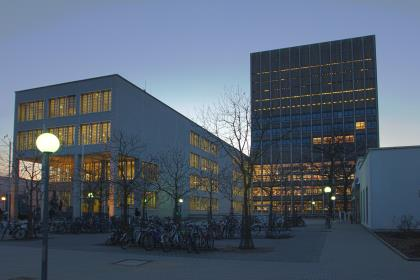
\includegraphics[width=\textwidth]{Figures/bib.jpg}
	\caption{Exterior view of the KIT library. Please always set images manually with the parameter [h]. At this point the image has been placed with the Figure parameter [h]. There is an empty line before and after the Figure environment.}
	\label{fig:bib}
\end{figure}

Lorem ipsum dolor sit amet, consetetur sadipscing elitr, sed diam nonumy eirmod tempor invidunt ut labore et dolore magna aliquyam erat, sed diam voluptua. At vero eos et accusam et justo duo dolores et ea rebum. Stet clita kasd gubergren, no sea takimata sanctus est Lorem ipsum dolor sit amet.

Curabitur a felis in nunc fringilla tristique. Morbi mattis ullamcorper velit. Phasellus gravida semper nisi. Nullam vel sem. Pellentesque libero tortor, tincidunt et, tincidunt eget, semper nec, quam. Sed hendrerit. Morbi ac felis. Nunc egestas, augue at pellentesque laoreet, felis eros vehicula leo, at malesuada velit leo quis pede. Donec interdum, metus et hendrerit aliquet, dolor diam sagittis ligula, eget egestas libero turpis vel mi. Nunc nulla. Fusce risus nisl, viverra et, tempor et.Pellentesque ut neque. Pellentesque habitant morbi tristique senectus et netus et malesuada fames ac turpis egestas. In dui magna, posuere eget, vestibulum et, tempor auctor, justo. In ac felis quis tortor malesuada pretium. Pellentesque auctor neque nec urna. Proin sapien ipsum, porta a, auctor quis, euismod ut, mi.

%\newpage
\begin{figure}[h] % "\begin{figure}" is an environment for floating objects, so that the figure can be numbered and labeled ("\caption{}") and provided with a label ("\label{fig:bib}") and referenced ("\ref{fig:bib} ")
	\centering
	%\hspace{-7pt} % Horizontal shift of the picture row
	\subfloat[Subfloat. Image No. 1. One-line captions are centered.]{%
		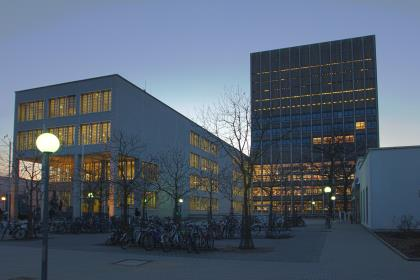
\includegraphics[width=0.49\linewidth]{Figures/bib.jpg}%
	}
	\hfill % Fills the vertical space between the images, provided the images are correspondingly small
	\subfloat[Subfloat. Image No. 2.]{%
		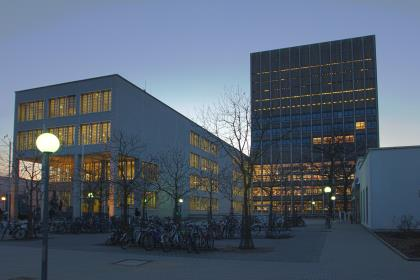
\includegraphics[width=0.49\linewidth]{Figures/bib.jpg}%
	}
	\\ \vspace{3mm} % Distance to the second row of images % plus distance due to the command "\captionsetup[subfloat]{belowskip=}" from the file dokOptions.tex
	%\hspace{-7pt} % Horizontal shift of the picture row
	\subfloat[Subfloat. Image No. 3. Note: If there are only two lines, the caption will not be justified as ragged right when using a manual line break.]{%
		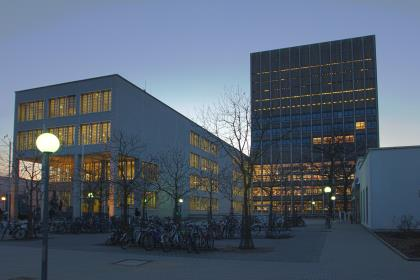
\includegraphics[width=0.49\linewidth]{Figures/bib.jpg}%
	}
	\hfill % Fills the vertical space between the images, provided the images are correspondingly small
	\subfloat[Subfloat. Image No. 4.]{%
		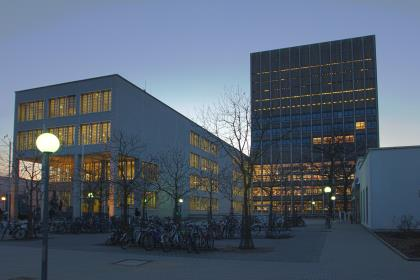
\includegraphics[width=0.49\linewidth]{Figures/bib.jpg}%
	}
	\caption{Exterior view of the KIT library. Please always set images manually with the parameter [h]. This is where the picture has been placed with the Figure parameter [h].}
	\label{fig:bib4}
\end{figure}

Aenean viverra rhoncus pede. Pellentesque habitant morbi tristique senectus et netus et malesuada fames ac turpis egestas. Ut non enim eleifend felis pretium feugiat vivamus quis mi. Phasellus a est. Phasellus magna. In hac habitasse platea dictumst. Curabitur at lacus ac velit ornare lobortis.\footnote{Cabo. Facerfe rferspient que nus molora doleserem. Ut a si autemo tectaquame enihil intota sam am ditati omnihil ma sequis re, aut fugiam earchil luptaque consequ.} Curabitur a felis in nunc fringilla tristique. Morbi mattis ullamcorper velit. Phasellus gravida semper nisi. Nullam vel sem. Pellentesque libero tortor, tincidunt et, tincidunt eget, semper nec, quam. Sed hendrerit.

%\newpage
Pellentesque habitant morbi tristique senectus et netus et malesuada fames ac turpis egestas. In dui magna, posuere eget, vestibulum et, tempor auctor, justo. In ac felis quis tortor malesuada pretium. Pellentesque auctor neque nec urna. Proin sapien ipsum, porta a, auctor quis, euismod ut, mi. Aenean viverra rhoncus pede. Pellentesque habitant morbi tristique senectus et netus et malesuada fames ac turpis egestas. Ut non enim eleifend felis pretium feugiat vivamus quis mi. Phasellus a est. Phasellus magna. In hac habitasse platea dictumst. Curabitur at lacus ac velit ornare lobortis. Aenean viverra rhoncus pede. Pellentesque habitant morbi tristique senectus et netus et malesuada fames ac turpis egestas. Ut non enim eleifend felis pretium feugiat vivamus quis mi. Phasellus a est. Phasellus magna. Phasellus a est. Phasellus magna. In hac habitasse platea dictumst. Curabitur at lacus ac velit ornare lobortis. Aenean viverra rhoncus pede. Pellentesque habitant morbi tristique senectus et netus et malesuada fames ac turpis egestas. Ut non enim eleifend felis pretium feugiat vivamus quis mi. Phasellus a est. Phasellus magna.

Phasellus magna. Phasellus a est. Phasellus magna. In hac habitasse platea dictumst. Curabitur at lacus ac velit ornare lobortis. Aenean viverra rhoncus pede. Pellentesque habitant morbi tristique senectus et netus et malesuada fames ac turpis egestas. Ut non enim eleifend felis pretium feugiat vivamus quis mi. Phasellus a est. Phasellus magna et netus et malesuada fames ac turpis egestas.

%\newpage
\begin{figure}[h]
	\centering
	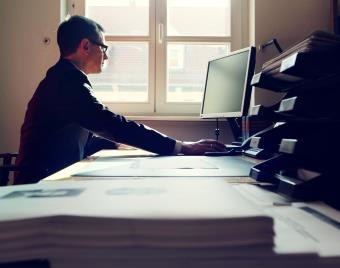
\includegraphics[width=6cm]{Figures/knowledge.jpg}
	\caption[Scientist in his workplace.] {Scientist in his workplace. Please always set images manually with the parameter [h]. At this point the image has been placed with the Figure parameter [h]. There is an empty line before and after the figure environment.}
	\label{fig:knowledge}
\end{figure}

Pellentesque habitant morbi tristique senectus et netus et malesuada fames ac turpis egestas. In dui magna, posuere eget, vestibulum et, tempor auctor, justo. In ac felis quis tortor malesuada pretium. Pellentesque auctor neque nec urna. Proin sapien ipsum, porta a, auctor quis, euismod ut, mi. Aenean viverra rhoncus pede. Pellentesque habitant morbi tristique senectus et netus et malesuada fames ac turpis egestas. Ut non enim eleifend felis pretium feugiat vivamus quis mi. Phasellus a est. Phasellus magna. In hac habitasse platea dictumst. Curabitur at lacus ac velit ornare lobortis.

Pellentesque habitant morbi tristique senectus et netus et malesuada fames ac turpis egestas. In dui magna, posuere eget, vestibulum et, tempor auctor, justo. In ac felis quis tortor malesuada pretium. Pellentesque auctor neque nec urna. Proin sapien ipsum, porta a, auctor quis, euismod ut, mi. Aenean viverra rhoncus pede. Pellentesque habitant morbi tristique senectus et netus et malesuada fames ac turpis egestas. Ut non enim eleifend felis pretium feugiat vivamus quis mi. Phasellus a est. Phasellus magna. In hac habitasse platea dictumst. Curabitur at lacus ac velit ornare lobortis. Pellentesque habitant morbi tristique senectus et netus et malesuada fames ac turpis egestas.

%Pellentesque habitant morbi tristique senectus et netus et malesuada fames ac turpis egestas. In dui magna, posuere eget, vestibulum et, tempor auctor. Pellentesque habitant morbi tristique senectus et netus et malesuada fames ac turpis egestas. In dui magna, posuere eget, vestibulum et, tempor auctor.

\begin{table}[h] % "\ begin {table}" is an environment for floating objects, so that the table "\ begin {tabular}" can be numbered, titled, labeled and referenced
	\caption{Tables are always inserted with the parameter [h].}
	\begin{tabularx}{\textwidth}{XXXXXXXX} \toprule
		Spalte1 & Spalte2 & Spalte3 & Spalte4 & Spalte5
		& Spalte6 & Spalte7 & Spalte8 \\ \midrule
		AA      & BB      & CC      & DD      &
		EE      & FF      & GG      & HH       \\
		AA      & BB      & CC      & DD
		& EE      & FF      & GG      & HH    \\
		AA      & BB      & CC      & DD
		& EE      & FF      & GG      & HH    \\
		AA      & BB      & CC      & DD
		& EE      & FF      & GG      & HH    \\
		AA      & BB      & CC      & DD
		& EE      & FF      & GG      & HH    \\
		AA      & BB      & CC      & DD
		& EE      & FF      & GG      & HH     \\ \bottomrule
	\end{tabularx}
\end{table}

Pellentesque habitant morbi tristique senectus et netus et malesuada fames ac turpis egestas. In dui magna, posuere eget, vestibulum et, tempor auctor. Pellentesque habitant morbi tristique senectus et netus et malesuada fames ac turpis egestas. In dui magna, posuere eget, vestibulum et, tempor auctor.